\chapter{Background}
In this section, we explain the background about the concepts and technologies imployed in the thesis. These includes the logic-based reasoning methods such as the Boolean satisfiability (SAT) and ontology-based on the description logic which are employed to improve quality of requirments specifications, the UPPAAL statistical model checking and stochastic time automata which is imployed in the formal analysis of Simulink models, and the integer-linear programming and metaheuristics optimization methods which are imployed in the resource optimization  in the software to hardware mapping.
\section{Logic-based Reasoning}
In this thesis, we express requirements specifications in  Boolean logic and apply Boolean satisfiability to detect inconsistencies in the specifications. Moreover, we apply ontology for a more rigoruous analysis of thes specifications.
\subsection*{Boolean Satisfiability (SAT)}
The study of a Boolean formula is generally concerned with the set of truth assignments (assignments of 0 or 1 to each of the variables) that make the formula true. Finding such assignments by answering the simpler question: ``does there exist a truth assignment that satisfies the boolean formula?'' is called the boolean satisfiability problem (SAT), which is proven to be NP complete. However, heuristics and approximation algorithms do exist to return the result. A SAT problem is formally defined as follows~\cite{devlin2008satisfiability}.

Z3 Theorem Prover/ SMT Solver. Satisfiability Modulo Theories (SMT)~\cite{Biere2009HandbookSatisfiability} is a decision problem expressed in the first-order logic which integrates a collection of background theories, e.g., on real numbers, bit vector, array, etc. SAT problems are usually described in terms of satisfiability, which is checked using decision procedures, known as SAT solvers. Z3 is a well-known SMT solver as well as a theorem prover developed by Microsoft Research which integrates several background theories and decision procedures using a DPLL- based SAT solver~\cite{DeMoura2008Z3:Solver}. It has been used in the formal verification and reasoning of software and hardware systems. Further, it has a strong support for integra- tion to verification tools using its well-known APIs, written in Java, Phyton, C++, C and .Net.

The Z3's input language is an extension of the SMT-LIB2 standard~\cite{SMT-LIB} which is used to assert formulas (expressions) as commands. The formulas can be checked for satisfiability using the command (check-sat). If the formulas are satisfiable, Z3 returns sat; if the formulas are not satisfiable, Z3 returns unsat, or if it cannot decide it returns unknown. In case of unsat, if the unsat-core option is enabled, Z3 returns the unsatisfiable subsets of assertions using the (get-unsat-core) command.

\subsection*{Ontology based on Description Logic}
Ontology is a knowledge-base representation method frequently used in the artificial intelligence and other areas to facitate decision making. Description Logic (DL)~\cite{Baader2010TheApplications} has its origins in the 1970s, and is intended to address the need for logical support to the representation of knowledge bases, mostly designed by using frames and semantic networks. Currently, the language is predominantly used in web semantics (e.g., OWL)~\cite{Rudi Studer, V Richard Benjamins, and Dieter Fensel. Knowledge En}, artificial intelligence~\cite{10.1007/978-94-017-9297-4_7}, bioinformatics~\cite{Rector2006}, software engineering, natural language pro- cessing. The language is designed with practicality in mind; consequently, it is usually backed by solid reasoning services that terminate and deliver results in reasonable time. The language uses Concepts (unary predicates), Roles (binary predicates) and Instances (logical symbols) that are recursively constructed us- ing Constructors. The most common constructor Subconcept (or concept inclu- sion) $\sqsubseteq$, is used to define concept hierarchies, and the equivalence constructor $\equiv$ defines the equivalence of concepts, through the bidirectional concept inclu- sions. Other basic constructors of the language include the conjunction (intersection) $\sqcap$, disjunction (union) $\sqcup$, the existential quantifier $\exists$, and the universal quantifier $\forall$. Currently, there are many variants of the language that differ in their expressivity. $\mathcal{sqsubseteq}$ (Attribute Language Complement) is considered the basis of the many Description Logic variants, for instance, $\mathcal{SROIQ}$ which is implemented in OWL 2 extends $\mathcal{ALC}$ (abbr. $\mathcal{S}$) with the role inclusion ($\mathcal{R}$), nominal ($\mathcal{O}$), inverse role ($\mathcal{I}$), qualified cardinality restrictions ($\mathcal{Q}$). 

%In this thesis, we use DL to represent the semantics of requirements spec-ifications using the notion of ontology. An ontology is a shared and reusable resource for knowledge-based systems. The requirements specifications are initially expressed in the constrained natural language ReSA. The benefit of this approach is the fact that it allows a deep analysis of requirements, not just at the syntactic level, but also on the semantics of the requirements statements that are expressed in a language that closely renders the syntax and semantics of natural language.
\section{Simulink Analysis}
Simulink~\cite{JamesB.Dabney2003MasteringSimulink} is a graphical development environment for the modeling, simulation and analysis of embedded systems which is widely used in industry to model and inspect the dynamics of systems before implementation. It is robust as it supports multi-domain, continuous, discrete, hybrid systems, also discrete systems that execute with different sampling times (or multi-rate). Figure~\ref{fig_sm_multi-rate} shows a multi-rate subsystem of the brake-by-wire Simulink model that models the brake pedal (i.e., continuous behaviror) and global brake functionality (i.e., discrete behavior), which executes every 10ms and 20ms.  
\begin{figure}[h]
	\centering
	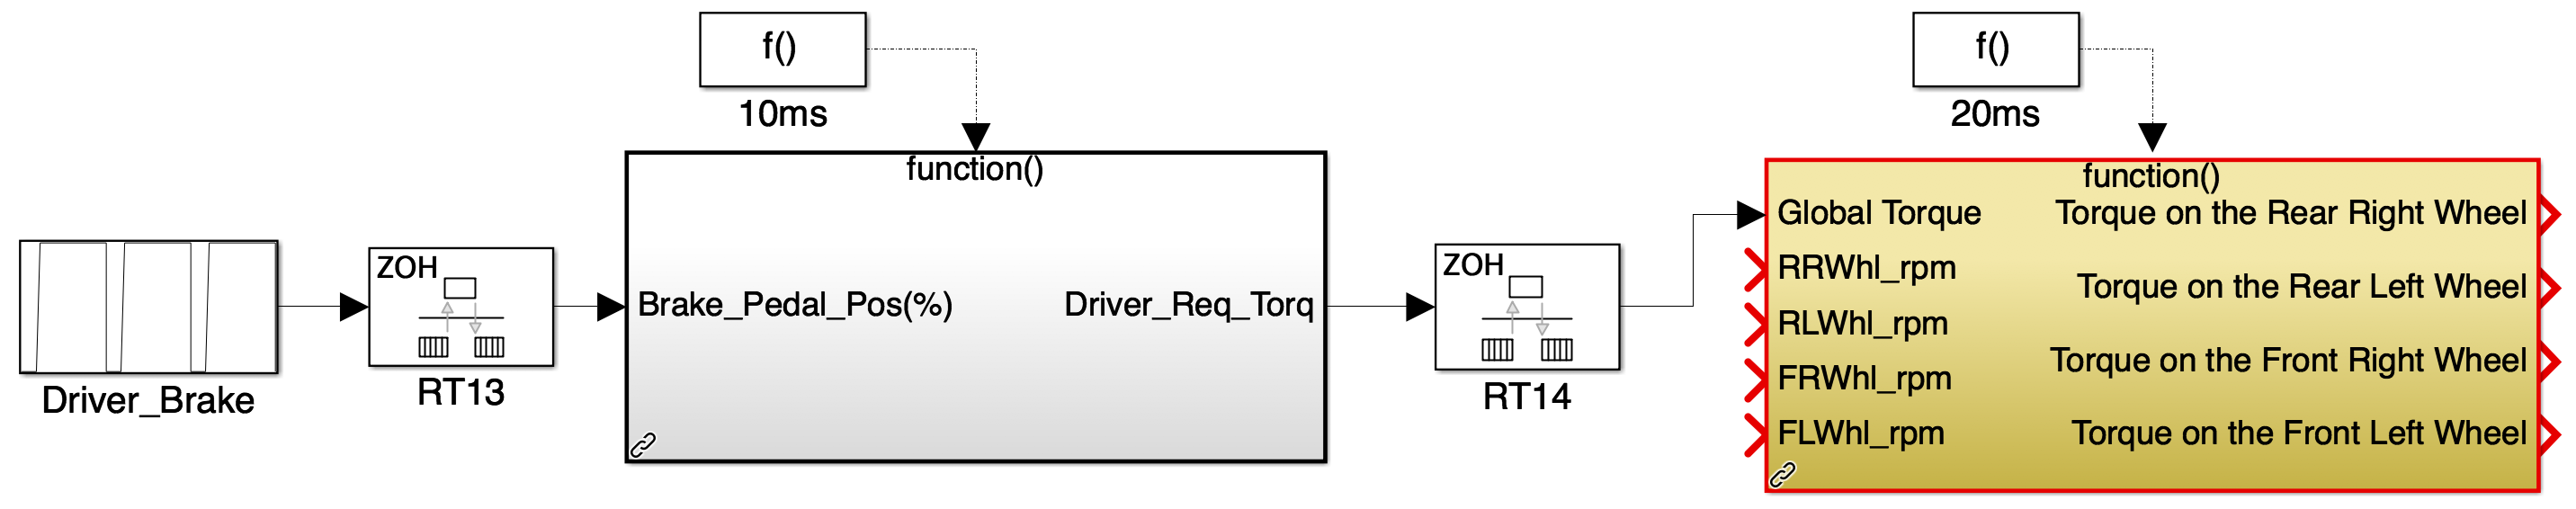
\includegraphics[width=0.9\linewidth]{images/sm}
	\caption{Brake pedal and global brake controller of the brake-by-wire model.}
	\label{fig_sm_multi-rate}
\end{figure}

Simulink is frequently used in the development of safey-critical systems, e.g., automotive, avionics, furthermore, it is used to generate code automatically from the models. Therefore, it is crucial that such models are analyzed rigorously. The Simuink Design Verifier (SDV) provides a formal verification technique that is based on the exact model checking to exhaustively verify functional properties~\cite{MathWokrksSimulinkVerifier}, however, its funtionality is limited as it lacks support for timed anlaysis, which is vital to ensure predictability of safety-critical embedded systems. 

\subsection*{Simulink Blocks}
A Simulink model is constructed from communicating function blocks (or Simulink blocks). The blocks implement simple to complex functionlity and consist of Input and Output ports, which enable communication via connectors. The latter modeling elements support basic and user-defined datatypes, e.g., integer, floating-point; and simple and complex data structures, e.g., scalar, vector, matrix.  Simulink blocks are classified into \textit{virtual} (non-computational, e.g., Mux, Demux blocks) and \textit{non-virtual} (computational, e.g., Gain, Integrator) blocks based on their computability. The non-virtual blocks improve the visualization of the model, but unlike the non-virtual blocks, they are not executed, hence do not affect the execution semantics of the model.  The blocks can be composed into groups, e.g., using Subsystem, Model blocks, to enable hierarchical modeling, which is used to improve the visualization, and to enforce execution order on a group of blocks. The fundamental constructs of the composite blocks are \textit{atomic} blocks, e.g., Gain, Sum blocks.

The non-virtual (computational) atomic blocks can be categorized into \textit{continuous} and \textit{discrete} blocks based on the execution semantics of the blocks.  A discrete block executes periodically with sample time $t_s$, whereas a continuous block executes over infinitesimal sample times. Since the Simulink blocks libraries are not usually sufficient to model practical embedded system systems, Simulink supports mechanisms to extend functionality that engineers can exploit to develop complex systems. The mechanisms include S-function, Custom Block and Masking. S-function is a computer language of Simulink blocks which allows advanced implementations of block routines, written in MATLAB, C, C++, or Fortran.


\subsection*{Execution of Simulink Blocks}
Duirng the initial phase of the simulation, the model is compiled, thus the order in which the blocks are executed is established known as \textit{sorted order} list. Figure~\ref{fig_sm_exec_order} shows the execution order via the labels in red color, annotated as $s:b$, where $s$ denotes the system/subsystem index and $b$ the block index\footnote{https://se.mathworks.com/help/simulink/ug/controlling-and-displaying-the-sorted-order.html}. Basically, the list is determined according to the data dependency of blocks' outputs on the blocks' input ports, i.e., if the output depends on the current value of the input, the input port is identified as \textit{direct-feedthrough} port. Thus, to preserver the data dependency in the model, the sort order rules require that the blocks that derive other blocks that have direct-feedthrough ports must come first in the list, e.g., blocks that derive Gain block. However, the blocks with non-direct-feedthrough ports, e.g., Delay block, can execute in any order, considering the previous rule. The execution order is also affected by the user defined priorities, neverthless, the priorites do not violate the rules. The sorted order list can be fetched by simulating the model in the debugging mode.
\begin{figure}
	\centering
	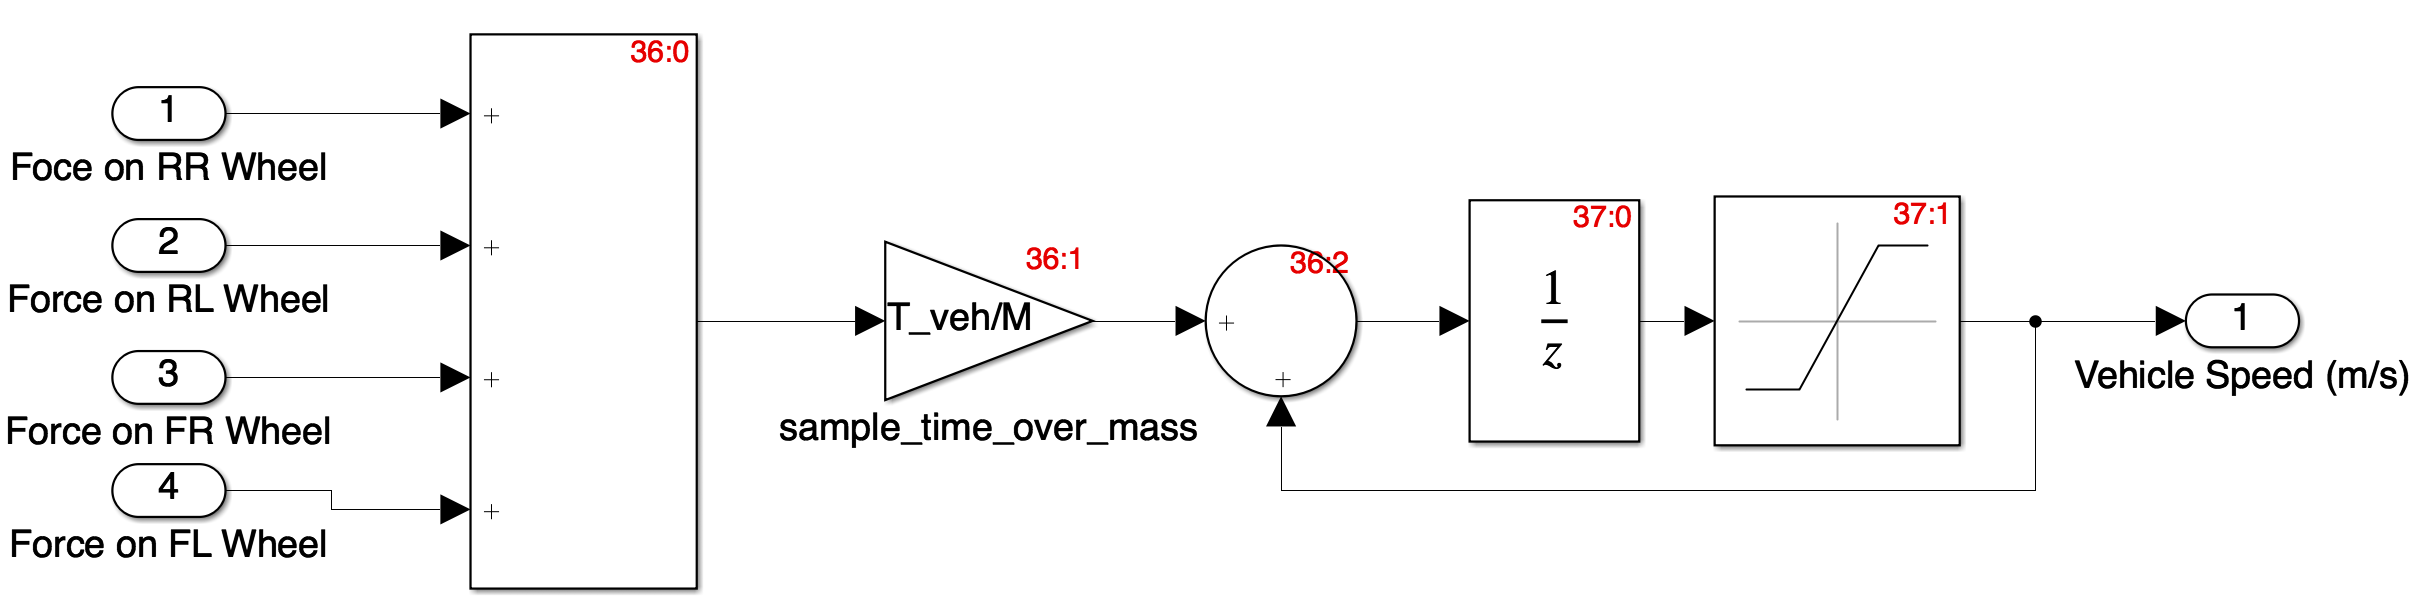
\includegraphics[width=1\linewidth]{images/sm_exec_order}
	\caption{A Subsystem block from the brake-by-wire model, computes vehicle speed. The labes in red color are indexed identifiers and denote of the execution order.}
	\label{fig_sm_exec_order}
\end{figure}

\section{UPPAAL Statistical Model Checking}
UPPAAL SMC \cite{david2012statistical} is a statistical model checker (implemented as an extension of \uppaal{} toolset) for system models represented as networks of stochastic priced timed automata. In \uppaalsmc{} the automata have a stochastic interpretation based on: (i) the probabilistic choices between multiple enabled transitions, and (ii) the non-deterministic time delays that can be refined based on probability distributions, either uniform distributions for time-bounded delays or user-defined exponential distributions for unbounded delays.

\section*{Stochastic Timed Automata}
A \textit{stochastic priced timed automaton} (SPTA) is defined as the following tuple:
\begin{equation}
SPTA=\langle L, l_0, X, \Sigma, E, R, I, \mu, \gamma \rangle,
\label{eq:STA}
\end{equation}
where
$L$ is a finite set of locations,
$l_0 \in L$ is the initial location,
$X$ is a finite set of continuous variables,
$\Sigma =\Sigma_i \uplus \Sigma_o$ is a finite set of actions partitioned into inputs ($\Sigma_i$) and outputs ($\Sigma_0$),
$E$ is a finite set of edges of the form $(l,g,a,\varphi, l')$, where $l$ and $l'$ are locations, $g$ is a predicate on
$\mathbb{R}^X$, action label $a \in \Sigma$, and $\varphi$ is a binary relation on $\mathbb{R}^X$, $R : L \rightarrow \mathbb{N}^X$ assigns a rate vector to each location,
$I$ assigns an invariant predicate $I(l)$ to any location $l$, $\mu$ is the set of all density delay functions $\mu_s \in L \times R^X$, which can be either uniform or exponential distribution, and $\gamma$ is the set of all output probability functions $\gamma_s$ over the $\Sigma_o$ output edges of the automaton.

The semantics of the probabilistic SPTA is defined over a timed transition system, whose states are pairs $s = (l,v) \in L \times \mathbb{R}^X$, with $v \models I(l)$, and transitions defined as:
(i) delay transitions ($(l, v)\xrightarrow{d}(l, v')$ with $d \in \mathbb{R}_{\geq 0}$ and $v'= v + d$), and
(ii) discrete transitions ($(l, v)\xrightarrow{a}(l', v')$ if there is an edge $(l,g,a,Y,l')$ such that $v \models g$ and $v'= v[Y]$, where $Y \subseteq X$, and $v[Y]$ is the valuation assigning 0 when $x \in Y$ and $v(x)$ otherwise).
We write $(l, v) \leadsto (l', v')$, if there is a finite sequence of delay and discrete transitions from $(l, v)$ to $(l', v')$. 
%The delay update for a simple clock $x$ is given by an implicit rate $x′=1$ or an explicit rate $x′=e$ appearing in the invariant of $l$, where $e$ is an expression only depending on the discrete part of the current state.
The delay density function $\mu_s$ over delays in $\mathbb{R}_{\geq 0}$ for each state $s$ is either a uniform or an exponential distribution, depending on the invariant of location $l$. Let $E_l$ denote the disjunction of guards such that $(l, g, o, -, -) \in E$ for some output $o$. Then, $D(l, v) = \mbox{sup}\{d \in \mathbb{R}_{\geq 0} : v + d \models I(l) \}$ denotes the supremum delay, whereas $d(l, v) = \mbox{inf}\{d \in \mathbb{R}_{\geq 0} : v + d \models  E_l \}$ denotes the infimum delay before enabling an output. If $D(l, v) < \infty$ then the delay density function $\mu_s$ for a given state $s$ is a uniform distribution over the interval $[d(l, v), D(l, v)]$, otherwise it is an exponential distribution with a rate $P(l)$. For every state $s$, the output probability function $\gamma_s$ over $\Sigma_o$ is a uniform distribution over the set $\{o : (l, g, o, -, -) \in E \land v \models g\}$ whenever the set is non empty. 

Under the assumption of input-enabledness, disjointedness of clock sets and output actions, a collection of composable SPTA can be defined as a  \textit{network of SPTA} (NSPTA), via the parallel composition operator ($A1\parallel A2 \parallel ... \parallel An$).
The states of the NSPTA are defined as a tuple $s = \langle s_1,...,s_n\rangle$, where $s_j$ is a state of $A_j$ of the form $(l, v)$, where $l \in L^j$ and $v \in \mathbb{R}^{X^j}$, where different automata synchronize based on standard broadcast channels. 
The probabilistic semantics is based on the principle of independence between components.
Each component decides on its own (based on a given delay density function and the output probability function) how much to delay before producing an output.

For encoding the patterns presented in this paper, we use SPTA with real-valued clocks that evolve with implicit rate 1. These automata are in fact timed automata with stochastic semantics, called \textit{stochastic timed automata} (STA). A \textit{network of STA} (NSTA) is a parallel composition of STA, defined in a similar way as NSPTA. The notion of SPTA is introduced due to the fact that, for analysis we use monitor automata (composed in parallel with the actual system model) that implement the \emph{stop-watch} mechanism, which renders the model a network of stop-watch timed automata, which is a subset of NSPTA.

\subsection*{Properties Specification}
\uppaalsmc{} uses a probabilistic extension of \textit{weighted metric temporal logic} (WMTL) \cite{bulychev2012rewrite} to provide:
\begin{itemize}
	\item \textit{Hypothesis testing}: check if the probability to reach a state $\phi$ within cost $x\leq C$ is greater or equal to a certain threshold $p$ ($Pr[<= bound](\star_{x\leq C}\phi) \geq p$),
	\item \textit{Probability evaluation}: calculate the probability $Pr[<= bound](\star_{x\leq C}\phi)$ for some NSPTA,
	\item \textit{Probability comparison}: is $Pr[<= bound](\star_{x\leq C}\phi_1) > Pr[<= bound](\star_{y\leq D}\phi_2)$?,
\end{itemize}
where $\star$ stands for either \textit{future} ($\Diamond$) or \textit{globally} ($\square$) temporal operator, and \textit{[<= bound]} denotes the time bound of the executions.
\section{Integer-linear Programming (ILP)}
\ilp{} is an optimization problem where the decision variables are integer, and the objective function and the constraints are linear models.  They are problems that can be represented as 
\begin{align}
	&Maximize\ \sum_{j=1}^{n}{c_jx_j}\\
	\mbox{Subjec to:}&\\
	&\sum_{j=1}^n{a_ijx_j}\leq b_i&\mbox{ for all } i=1,...,m\\
	&x_j\geq 0 \land x_i\in \mathbb{I} &\mbox{ for all } i=1,...,m
\end{align}

It has many mathematical, and engineering applications, e.g., transportation, scheduling. The binary (0-1) problem is a special case of ILP where the decions variables takes on 0 or 1. It appied in several decision making problems, e.g., resource allocation in the scheduling/ assignment problem. The software mapping is an instance the assignment problem where each binary variable denote if a software component is mapped to a  processor (or computing unit) or not, i.e., 1 if assigned otherwise 0. 

ILP problems are frequenlty solved via exact algorithms, e.g., branch and bound, but can also be delt via heuristics, e.g., using simulated annealing, hill climbing. In this work, we use the CPLEX solver form IBM to the software-to-hardware mapping optimization.
\section{Population-based Metaheuristics}
For complex optimization problems, the ILP formulation is a difficult task and the scalability to solve large problems instances is usually prohobitively expensive. Metaheuristics is a type of heuristics which uses search strategies that are sometimes less dependent on the problems and more efficient computation-wise but less optimal. Population-based metaheuristics is a class of meta-heuristic methods which uses a set of individuals (or population) in the search strategy to determine the global optima of the problem, e.g., genetic algorith, differential evolution, particle swarm optimization.

In this work, we apply differential evolution, particle-swarm optimization to search for the best software-to-hardware mapping solution. The differential evolution employes a set of agents, which represent candidate solutions,  to find the best software-to-hardware mapping solution. Each agent applies a particular types of evolutionary operators such as mutation, crossover and selection to reach a target position in the search space. A mutant agent (or offspring) is generated for every agent and in every iteration from three other angents. If the offspring is more fit, i.e., better than the parent agent, it replaces the latter, otherwise is discarded.
\begin{align}
\label{eqn_de_mutation}
\textbf{v} & \leftarrow   \textbf{a} + F\circ(\textbf{b}-\textbf{c})\\
\label{eqn_de_crossover}
\textbf{u}&\leftarrow crossOver(\textbf{v},\textbf{x},CF,F)\\
\label{eqn_de_selection}
\textbf{x} &\leftarrow 
\begin{cases}
	\textbf{u} & \mbox{if } f(\textbf{u}) < f(\textbf{x})\mbox{ functions}\\
	\textbf{x} & \mbox{otherwise }
\end{cases}
\end{align}
where $F\in[0,2]$ is the differential weight, $CF\in[0,1]$ is the crossover probability.

Likewise, in the particle-swarm optimization, the method employs agents (in this case, particles), which are memeber of the population and represents candidate solutions. It records the best position of each particle so far $\textbf{p}_{bst}$ and best position of the population $\textbf{z}$. Thus, the motion of each particle is guided by its velocity, attraction towards its best position $\textbf{p}_{bst}-\textbf{p}$ and attraction towards the best position of the swarm $\textbf{z}-\textbf{p}$, where $\textbf{p}$ is a n-dimensional matrix which represents the current position of a particle in the search space.
\begin{align}
\label{eqn_pso_velocity}
\textbf{v} &\leftarrow  \omega\textbf{v} + c_1Rand()\circ(\textbf{p}_{bst}-\textbf{p}) + c_2Rand()\circ(\textbf{z}-\textbf{p})\\
\label{eqn_pso_position}
\textbf{p} &\leftarrow \textbf{p} + \textbf{v},
\end{align}
where $\omega$ is the weight of the velocity, also known as \textit{inertia coefficient} and controls the convergence of the algorithm. The $c_1, c_2$ constants are acceleration coefficients and control the weight of attraction towards the cognitive and social components, respectively. $Rand()\in U(0,1)$ is a random function along the acceleration coefficients, which is element-wise multiplied with the components to improve diversity of the search by introducing stochastic behavior.